\documentclass[10pt,twocolumn,letterpaper]{article}

\usepackage[margin=0.75in]{geometry}
\usepackage{amsmath,amssymb,amsfonts,amsthm}
\usepackage{booktabs}
\usepackage{graphicx}
\usepackage{microtype}
\usepackage{hyperref}
\usepackage{xcolor}
\usepackage{algorithm}
\usepackage{algpseudocode}
\usepackage{cite}

\hypersetup{
    colorlinks=true,
    linkcolor=blue!70!black,
    citecolor=blue!70!black,
    urlcolor=blue!80!black
}

\newtheorem{theorem}{Theorem}
\newtheorem{proposition}{Proposition}
\newtheorem{lemma}{Lemma}
\newtheorem{definition}{Definition}
\newtheorem{corollary}{Corollary}

\title{\textbf{CentroidSteer: Activation-Guided Low-Rank Subspace Optimization on the Stiefel Manifold for Sparse Mixture-of-Experts}}

\author{
    \textbf{Yash Bhardwaj} \\
    Triune AI \\
    \texttt{yash@triune.ai}
}

\date{\today}

\begin{document}

\maketitle

\begin{abstract}
First-order adaptive optimizers such as AdamW maintain persistent first and second gradient moments that consume $8.0$ bytes of high-bandwidth memory (HBM) per parameter, constituting a primary bottleneck in scaling modern foundation models. While low-rank gradient projection methods mitigate optimizer memory, they project updates onto arbitrary principal directions that ignore the dynamic activation geometry of routed expert tokens in sparse Mixture-of-Experts (MoE) architectures. Furthermore, recent matrix polar optimization methods (such as Muon) treat parameter tensors uniformly, causing empirical instability when applied indiscriminately to high-aspect-ratio vocabulary embeddings. In this paper, we propose \textbf{CentroidSteer}, a mathematically grounded, activation-guided, tri-tier partitioned optimizer operating on the compact Stiefel manifold for sparse MoE architectures. CentroidSteer dynamically partitions weights into: (1) \textbf{Tier 1} (Muon), applying 5th-order Newton-Schulz polar orthogonalization to 2D attention matrices; (2) \textbf{Tier 2} (CentroidSteer), projecting routed expert updates into an augmented low-rank subspace steered along empirical router activation centroids and retracting onto the Stiefel manifold $\operatorname{St}(r+1, d)$ via two-pass shifted Cholesky-QR Gram orthogonalization; and (3) \textbf{Tier 3} (Base AdamW), preserving 1D normalization layers, router gates, and vocabulary embeddings under standard fused adaptive updates. Mathematically, we prove that alternating orthogonal subspace iteration combined with activation augmentation produces an exact upper-triangular block Krylov core $\bar{S} = \bar{Q}_L^T G \bar{Q}_R$, establishing the theoretical validity of the triangular projection without discarding legitimate gradient information. We further prove that router gating entropy $\mathcal{H}(p)$ strictly bounds the intra-cluster activation dispersion and residual subspace perturbation, establishing a formal connection between routing certainty and subspace alignment. In multi-seed pre-training evaluations on FineWeb-Edu ($N=3$ seeds from scratch; $N=12$ seeds, $df=11$, $200$ steps from a 75.8M 6-layer Studio checkpoint at step $36,500$ [$222.7\text{M}$ tokens] across balanced $3 \times 3$ Latin squares), CentroidSteer reduces persistent expert optimizer memory by $98.4\%$ to \textbf{0.128} bytes/param ($4.54$ bytes/param model-wide with standard Tier 3 AdamW, or $1.27$ bytes/param with 8-bit AdamW) and demonstrates equivalence within $\pm 0.01$ nats ($p_{\text{TOST}} = 1.52 \times 10^{-7}$), establishing its viability as an activation-informed inductive prior without degradation.
\end{abstract}

\section{Introduction}

Scaling autoregressive large language models is fundamentally constrained by GPU memory capacity and memory bandwidth during distributed pre-training~\cite{kaplan2020scaling,radford2019language}. While activation memory can be managed via activation checkpointing and selective rematerialization~\cite{chen2016training}, optimizer states—specifically the first and second moments ($m_t, v_t$) required by AdamW~\cite{loshchilov2017decoupled,kingma2014adam}—must remain permanently resident in memory. In single-device and distributed data-parallel training, these auxiliary states consume $8$ bytes per parameter in standard FP32 precision, often dwarfing the footprint of the underlying model weights ($2$ bytes in BF16) and limiting the maximum trainable parameter budget.

To mitigate this memory overhead, low-rank projection frameworks such as GaLore~\cite{zhao2024galore} and BAdam~\cite{liu2024badam} demonstrate that gradient updates often reside on slowly drifting, low-dimensional manifolds. However, existing low-rank projection techniques present two central deficiencies when applied to modern Mixture-of-Experts (MoE) architectures~\cite{shazeer2017outrageously,fedus2022switch,jiang2024mixtral,deepseek2024v3}:
\begin{enumerate}
    \item \textbf{Decoupling from Token Routing Manifolds}: In sparse MoE layers, tokens are dynamically partitioned across experts based on router gate affinities. Each expert processes a clustered subset of the activation distribution. Standard low-rank gradient projection projects expert gradients solely onto singular vectors of the unweighted parameter gradient, disregarding the geometric cluster centroid of the tokens that the expert actually processed.
    \item \textbf{Uniform Treatment of Heterogeneous Weight Tensors}: Recent matrix polar optimization techniques, such as Muon~\cite{jordan2024muon}, accelerate training by equalizing singular values across hidden weight matrices. However, applying singular value equalization uniformly across a model degrades vocabulary embeddings and unembedding heads ($\text{vocab} \gg d$), which require anisotropic, frequency-dependent coordinate representations.
\end{enumerate}

To address these challenges, we introduce \textbf{CentroidSteer}, a mathematically rigorous optimization framework specifically designed for sparse MoE architectures. CentroidSteer introduces six primary contributions:
\begin{itemize}
    \item \textbf{Riemannian Geometry on the Stiefel Manifold}: We formulate low-rank subspace updates within the Riemannian geometry of the compact Stiefel manifold $\operatorname{St}(r, d)$, deriving tangent space projections and computationally efficient polar Cholesky and Cayley geodesic retractions that eliminate manifold drift.
    \item \textbf{Tri-Tier Parameter Partitioning}: We introduce a principled parameter role taxonomy that separates 2D attention projections (Tier 1: Polar Orthogonalization), routed expert MLP matrices (Tier 2: Activation-Guided Subspace), and sensitive embeddings/normalizations (Tier 3: Fused AdamW).
    \item \textbf{Activation-Guided Subspace Steering}: We augment the low-rank gradient projection basis with the empirical activation centroid of tokens assigned to each expert, mathematically proving that the augmented basis remains strictly orthonormal and provides robust rank-deficient fallbacks.
    \item \textbf{Augmented Krylov Core Triangularization}: We prove that alternating orthogonal subspace iteration and activation centroid augmentation naturally yield an exact block upper-triangular projection core $\bar{S} = \bar{Q}_L^T G \bar{Q}_R = \begin{bmatrix} R_L & Q_L^T G \tilde{v}_\perp \\ \mathbf{0} & \tilde{c}_\perp^T G \tilde{v}_\perp \end{bmatrix}$, establishing that strictly lower-triangular entries are algebraically zero and resolving the theoretical validity of triangular core updates.
    \item \textbf{Routing Entropy Concentration Bounds}: We prove that the Shannon entropy of token routing probabilities strictly bounds the intra-cluster activation dispersion and residual subspace perturbation, establishing a rigorous connection between expert specialization and low-rank alignment.
    \item \textbf{Two-Pass Shifted Cholesky-QR Stability \& Convergence}: We prove the unconditional orthogonal stability of two-pass shifted Cholesky-QR (\texttt{sCholQR2}) under shift regularization and establish the non-convex convergence of Riemannian CentroidSteer on smooth objectives.
\end{itemize}

\section{Riemannian Geometry of the Stiefel Manifold \& Retractions}

\subsection{The Stiefel Manifold and Tangent Bundle}

In low-rank subspace optimization, the left and right projection bases $Q_L \in \mathbb{R}^{m \times r}$ and $Q_R \in \mathbb{R}^{n \times r}$ must maintain mutually orthonormal columns at all training steps. Geometrically, each basis matrix resides on the compact \textbf{Stiefel manifold}~\cite{edelman1998geometry,absil2008optimization}:
\begin{equation}
    \operatorname{St}(r, d) = \left\{ Q \in \mathbb{R}^{d \times r} \;\middle|\; Q^T Q = I_r \right\}, \quad (r \le d)
\end{equation}
The Stiefel manifold $\operatorname{St}(r, d)$ is an embedded Riemannian submanifold of $\mathbb{R}^{d \times r}$ with dimension $\operatorname{dim}(\operatorname{St}(r, d)) = d r - \frac{1}{2} r (r+1)$. We equip $\operatorname{St}(r, d)$ with the canonical Riemannian metric inherited from the Euclidean ambient inner product:
\begin{equation}
    \langle \xi, \eta \rangle_Q = \operatorname{tr}\left( \xi^T \eta \right), \quad \forall \; \xi, \eta \in T_Q \operatorname{St}(r, d)
\end{equation}
Differentiating the orthonormality constraint $Q(t)^T Q(t) = I_r$ with respect to $t$ shows that any tangent vector $\xi \in T_Q \operatorname{St}(r, d)$ satisfies:
\begin{equation}
    Q^T \xi + \xi^T Q = \mathbf{0}_{r \times r}
\end{equation}
Thus, $Q^T \xi$ must be a skew-symmetric matrix in $\mathfrak{so}(r)$. The tangent space at $Q$ decomposes into normal and tangent components:
\begin{equation}
    T_Q \operatorname{St}(r, d) = \left\{ \xi \in \mathbb{R}^{d \times r} \;\middle|\; Q^T \xi \in \mathfrak{so}(r) \right\}
\end{equation}

\begin{proposition}[Orthogonal Tangent Projection]
Let $Z \in \mathbb{R}^{d \times r}$ be an arbitrary ambient matrix. The orthogonal projection $\mathcal{P}_{T_Q}: \mathbb{R}^{d \times r} \to T_Q \operatorname{St}(r, d)$ under the canonical metric is given by:
\begin{align}
    \mathcal{P}_{T_Q}(Z) &= Z - Q \operatorname{sym}(Q^T Z) \nonumber \\
    &= (I - Q Q^T) Z + Q \operatorname{skew}(Q^T Z) \label{eq:tangent_proj}
\end{align}
where $\operatorname{sym}(M) = \frac{1}{2}(M + M^T)$ and $\operatorname{skew}(M) = \frac{1}{2}(M - M^T)$.
\end{proposition}

\begin{proof}
Let $\xi = Z - Q \operatorname{sym}(Q^T Z)$. We verify membership in $T_Q \operatorname{St}(r, d)$:
\begin{align}
    Q^T \xi &= Q^T Z - Q^T Q \operatorname{sym}(Q^T Z) = Q^T Z - \operatorname{sym}(Q^T Z) \nonumber \\
    &= Q^T Z - \frac{1}{2}(Q^T Z + Z^T Q) = \frac{1}{2}(Q^T Z - Z^T Q) \in \mathfrak{so}(r)
\end{align}
For any $\eta \in T_Q \operatorname{St}(r, d)$, $Q^T \eta + \eta^T Q = \mathbf{0}$, which implies $\operatorname{sym}(Q^T \eta) = \mathbf{0}$. Therefore:
\begin{equation}
    \langle Z - \xi, \eta \rangle = \operatorname{tr}\left( \operatorname{sym}(Q^T Z)^T Q^T \eta \right) = 0
\end{equation}
since the trace of the product of a symmetric matrix and a skew-symmetric matrix is identically zero. Thus $\xi$ is the unique orthogonal projection.
\end{proof}

\subsection{Geodesic Retractions onto the Stiefel Manifold}

During optimization, taking a step along a tangent vector $\xi \in T_Q \operatorname{St}(r, d)$ departs from the manifold due to curvature. A \textbf{retraction} $\mathcal{R}_Q: T_Q \operatorname{St}(r, d) \to \operatorname{St}(r, d)$ is a smooth mapping satisfying:
\begin{enumerate}
    \item $\mathcal{R}_Q(\mathbf{0}) = Q$,
    \item The differential $D \mathcal{R}_Q(\mathbf{0})$ is the identity mapping on $T_Q \operatorname{St}(r, d)$ ($D \mathcal{R}_Q(\mathbf{0})[\xi] = \xi$).
\end{enumerate}

\paragraph{Geodesic Exponential Mapping} The exact geodesic curve on $\operatorname{St}(r, d)$ emanating from $Q$ in direction $\xi$ under the Euclidean metric is given by Edelman et al.~\cite{edelman1998geometry}:
\begin{equation}
    \operatorname{Exp}_Q(t \xi) = \begin{bmatrix} Q & U \end{bmatrix} \exp \left( t \begin{bmatrix} A & -R^T \\ R & \mathbf{0} \end{bmatrix} \right) \begin{bmatrix} I_r \\ \mathbf{0} \end{bmatrix} \label{eq:geodesic}
\end{equation}
where $A = Q^T \xi \in \mathfrak{so}(r)$, and $U R = (I - Q Q^T) \xi$ is the thin QR decomposition of the normal component of $\xi$. While theoretically exact, evaluating the $2r \times 2r$ matrix exponential in Eq.~\eqref{eq:geodesic} at every optimizer step is computationally demanding.

\paragraph{Polar Cholesky Retraction} CentroidSteer replaces the geodesic exponential with the computationally optimal \textbf{Polar Cholesky Retraction}:
\begin{equation}
    \mathcal{R}_Q^{\text{polar}}(\xi) = (Q + \xi) \left( (Q + \xi)^T (Q + \xi) \right)^{-1/2} = (Q + \xi) L^{-T} \label{eq:polar_retraction}
\end{equation}
where $L L^T = (Q + \xi)^T (Q + \xi) + \epsilon_{\text{shift}} I_r$ is the lower-triangular Cholesky factor of the Gram matrix. 

\begin{proposition}[Retraction Properties of Polar Cholesky Mapping]
The mapping $\mathcal{R}_Q^{\text{polar}}$ defined in Eq.~\eqref{eq:polar_retraction} is a valid first-order retraction on $\operatorname{St}(r, d)$ and satisfies $\left( \mathcal{R}_Q^{\text{polar}}(\xi) \right)^T \mathcal{R}_Q^{\text{polar}}(\xi) = I_r$ with computational complexity $\mathcal{O}(d r^2 + r^3)$.
\end{proposition}

\begin{proof}
Let $Y = Q + \xi$. If $Y$ has full column rank $r$, then $Y^T Y$ is symmetric positive definite with unique factor $L L^T = Y^T Y$. Then:
\begin{equation}
    (Y L^{-T})^T (Y L^{-T}) = L^{-1} (Y^T Y) L^{-T} = L^{-1} (L L^T) L^{-T} = I_r
\end{equation}
Thus $\mathcal{R}_Q^{\text{polar}}(\xi) \in \operatorname{St}(r, d)$. At $\xi = \mathbf{0}$, $Y = Q$, $Q^T Q = I_r$, $L = I_r$, so $\mathcal{R}_Q^{\text{polar}}(\mathbf{0}) = Q$.
Differentiating $Y(t) = Q + t \xi$ at $t = 0$:
\begin{equation}
    \left. \frac{d}{dt} \mathcal{R}_Q^{\text{polar}}(t \xi) \right|_{t=0} = \xi - Q \operatorname{sym}(Q^T \xi)
\end{equation}
Since $\xi \in T_Q \operatorname{St}(r, d)$, $Q^T \xi \in \mathfrak{so}(r)$, so $\operatorname{sym}(Q^T \xi) = \mathbf{0}$. Therefore, $D \mathcal{R}_Q^{\text{polar}}(\mathbf{0})[\xi] = \xi$, verifying both retraction conditions.
\end{proof}

\paragraph{Cayley Transform Retraction for 2D Parameters} For full-rank 2D parameter matrices $W \in \mathbb{R}^{m \times n}$ ($m \le n$) under unitary manifold optimization (matching \texttt{UnitaryManifoldOptimizer}), let $\Omega = \frac{1}{\|W\|_F^2} (M W^T - W M^T) \in \mathfrak{so}(m)$ denote the skew-symmetric momentum operator. The Cayley retraction:
\begin{equation}
    \mathcal{R}_W^{\text{Cayley}}(M) = \left( I_m - \frac{\eta}{2} \Omega \right)^{-1} \left( I_m + \frac{\eta}{2} \Omega \right) W \label{eq:cayley}
\end{equation}
preserves exact row isometry $W_{t+1} W_{t+1}^T = W_t W_t^T = I_m$ unconditionally without requiring SVD or square root operations.

\section{CentroidSteer Formulation}

\subsection{Tri-Tier Parameter Partitioning}

Let $\Theta = \{\theta_i\}_{i=1}^P$ denote the parameters of a Mixture-of-Experts transformer. We partition $\Theta$ into three mutually exclusive functional tiers:
\begin{equation}
    \Theta = \Theta_{\text{Tier 1}} \cup \Theta_{\text{Tier 2}} \cup \Theta_{\text{Tier 3}}, \quad \Theta_i \cap \Theta_j = \emptyset \; (i \neq j)
\end{equation}

\begin{definition}[Parameter Role Taxonomy]
\begin{itemize}
    \item \textbf{Tier 1} ($\Theta_{\text{Tier 1}}$, Muon): 2D linear weights in dense attention mechanisms (query, key, value, output projections) and shared expert feed-forward matrices.
    \item \textbf{Tier 2} ($\Theta_{\text{Tier 2}}$, CentroidSteer): 2D and 3D routed expert matrices $\{W_1^{(e)}, W_2^{(e)}, W_3^{(e)}\}_{e=1}^E$ where $E$ is the number of routed experts.
    \item \textbf{Tier 3} ($\Theta_{\text{Tier 3}}$, Base AdamW): 1D parameters (RMSNorm scales, biases), router gating matrices $W_{\text{gate}}$, and large vocabulary matrices ($W_{\text{embed}}, W_{\text{head}}$).
\end{itemize}
\end{definition}

Explicit precedence rules enforce that vocabulary embeddings—identified via module type (\texttt{nn.Embedding}), pointer tie checks, or aspect ratio ($\text{dim}_0 / \text{dim}_1 \ge 4.0$ with $\text{dim}_0 \ge 1000$)—are unconditionally routed to Tier 3.

\subsection{Alternating Subspace QR and the Triangular Core}

For an expert weight matrix $W \in \mathbb{R}^{m \times n}$ with stochastic gradient $G \in \mathbb{R}^{m \times n}$, we assume $m \le n$ without loss of generality. Standard two-sided subspace methods project $G$ into an $r$-dimensional left subspace $Q_L \in \mathbb{R}^{m \times r}$ and right subspace $Q_R \in \mathbb{R}^{n \times r}$.

To construct $Q_L$ and $Q_R$ with minimal computational latency, CentroidSteer performs alternating subspace iterations with a Gaussian test matrix $\Omega \in \mathbb{R}^{n \times r}$:
\begin{align}
    Y_0 &= G \Omega \in \mathbb{R}^{m \times r}, & Q_L^{(0)} &= \text{CholQR}(Y_0) \\
    Z &= G^T Q_L^{(0)} \in \mathbb{R}^{n \times r}, & Q_R &= \text{CholQR}(Z) \\
    Y &= G Q_R \in \mathbb{R}^{m \times r}, & Q_L, R_L &= \text{QR}(Y) \label{eq:ql_qr}
\end{align}

Here, $\text{CholQR}(Y)$ denotes Two-Pass Shifted Cholesky-QR (\texttt{sCholQR2}):
\begin{align}
    \tilde{Y} &= Y \cdot \operatorname{diag}(\|y_1\|_2^{-1}, \dots, \|y_r\|_2^{-1}), \nonumber \\
    A_1 &= \tilde{Y}^T \tilde{Y} + \epsilon_{\text{shift}} I_r = L_1 L_1^T, \quad Q_1 = \tilde{Y} L_1^{-T} \\
    \hat{Q}_1 &= Q_1 \cdot \operatorname{diag}(\|q_{1,1}\|_2^{-1}, \dots, \|q_{1,r}\|_2^{-1}), \nonumber \\
    A_2 &= \hat{Q}_1^T \hat{Q}_1 + \epsilon_{\text{shift}} I_r = L_2 L_2^T, \quad Q = \hat{Q}_1 L_2^{-T}
\end{align}
where $\epsilon_{\text{shift}} = 10^{-7}$ in both passes under standard 32-bit floating-point precision (matching \texttt{triune/ops/centroid\_steer.py}).

\subsection{Dynamic Router Centroid Steering}

During forward evaluation of an MoE layer with router gate $g(x)$, let $\mathcal{S}_e = \{i \mid e \in \text{Top-}k(g(x_i))\}$ denote the batch tokens assigned to expert $e$. The layer router computes the empirical activation centroid:
\begin{equation}
    c_e = \frac{1}{|\mathcal{S}_e|} \sum_{i \in \mathcal{S}_e} x_i \in \mathbb{R}^m
\end{equation}
To steer expert parameter updates along this active functional manifold without perturbing existing gradient principal directions, we project $c_e$ into the orthogonal complement of the left basis $Q_L$:
\begin{equation}
    c_\perp = (I - Q_L Q_L^T) c_e
\end{equation}

We evaluate numerical stability thresholds before augmentation:
\begin{equation}
    \tilde{c}_\perp = \begin{cases} 
        \frac{c_\perp}{\|c_\perp\|_2}, & \text{if } \|c_\perp\|_2 > \tau \\
        \mathbf{0}_{m \times 1}, & \text{otherwise}
    \end{cases}
\end{equation}
with threshold $\tau = 10^{-8}$. To construct the corresponding right dual steering vector, we evaluate the gradient action:
\begin{equation}
    v = G^T \tilde{c}_\perp, \quad v_\perp = (I - Q_R Q_R^T) v
\end{equation}
\begin{equation}
    \tilde{v}_\perp = \begin{cases}
        \frac{v_\perp}{\|v_\perp\|_2}, & \text{if } \|c_\perp\|_2 > \tau \text{ and } \|v_\perp\|_2 > \tau \\
        \mathbf{0}_{n \times 1}, & \text{otherwise}
    \end{cases}
\end{equation}

When both stability thresholds pass ($\|c_\perp\|_2 > \tau$ and $\|v_\perp\|_2 > \tau$), the projection bases are augmented to rank $r+1$:
\begin{equation}
    \bar{Q}_L = [Q_L, \; \tilde{c}_\perp] \in \mathbb{R}^{m \times (r+1)}, \quad \bar{Q}_R = [Q_R, \; \tilde{v}_\perp] \in \mathbb{R}^{n \times (r+1)}
\end{equation}

\section{Theoretical Analysis \& Rigorous Proofs}

\begin{proposition}[Basis Isometricity and Rank Fallback]
\label{prop:ortho}
Let $Q_L \in \mathbb{R}^{m \times r}$ and $Q_R \in \mathbb{R}^{n \times r}$ have orthonormal columns ($Q_L^T Q_L = I_r, Q_R^T Q_R = I_r$).
\begin{enumerate}
    \item When $\|c_\perp\|_2 > \tau$ and $\|v_\perp\|_2 > \tau$, the augmented bases $\bar{Q}_L$ and $\bar{Q}_R$ are exact isometric embeddings on $\operatorname{St}(r+1, m)$ and $\operatorname{St}(r+1, n)$ satisfying $\bar{Q}_L^T \bar{Q}_L = I_{r+1}$ and $\bar{Q}_R^T \bar{Q}_R = I_{r+1}$.
    \item When either stability threshold fails, $\tilde{c}_\perp = \mathbf{0}$ and $\tilde{v}_\perp = \mathbf{0}$. The effective rank of the projection bases strictly falls back from $r+1$ to $r$, guaranteeing that the update is confined entirely to the unperturbed Krylov subspace $\operatorname{span}(Q_L) \times \operatorname{span}(Q_R)$ without division-by-zero or numerical degeneracy.
\end{enumerate}
\end{proposition}

\begin{proof}
For part (1), let $q \in \operatorname{col}(Q_L)$ such that $q = Q_L a$ for $a \in \mathbb{R}^{r}$. Then:
\begin{equation}
    q^T c_\perp = a^T Q_L^T (I - Q_L Q_L^T) c_e = a^T (Q_L^T - Q_L^T Q_L Q_L^T) c_e = 0
\end{equation}
because $Q_L^T Q_L = I_r$. Normalizing by $\|c_\perp\|_2 > 0$ preserves orthogonality: $Q_L^T \tilde{c}_\perp = \mathbf{0}_{r \times 1}$. Combined with $\|\tilde{c}_\perp\|_2 = 1$, we obtain:
\begin{equation}
    \bar{Q}_L^T \bar{Q}_L = \begin{bmatrix} Q_L^T Q_L & Q_L^T \tilde{c}_\perp \\ \tilde{c}_\perp^T Q_L & \tilde{c}_\perp^T \tilde{c}_\perp \end{bmatrix} = \begin{bmatrix} I_r & \mathbf{0} \\ \mathbf{0}^T & 1 \end{bmatrix} = I_{r+1}
\end{equation}
Identical reasoning applies to $v_\perp = (I - Q_R Q_R^T) v$, establishing that $Q_R^T \tilde{v}_\perp = \mathbf{0}_{r \times 1}$ and $\bar{Q}_R^T \bar{Q}_R = I_{r+1}$.
For part (2), setting column $r+1$ to zero yields $\bar{Q}_L \bar{Q}_L^T = Q_L Q_L^T$ and $\bar{Q}_R \bar{Q}_R^T = Q_R Q_R^T$, so the effective rank is identically $r$.
\end{proof}

\begin{theorem}[Augmented Upper-Triangular Subspace Identity]
\label{thm:augmented_triu}
Let $Q_R \in \mathbb{R}^{n \times r}$ have orthonormal columns ($Q_R^T Q_R = I_r$), and let $(Q_L, R_L) = \operatorname{qr}(G Q_R)$ be the thin QR decomposition of $G Q_R$ such that $G Q_R = Q_L R_L$ with $Q_L^T Q_L = I_r$ and $R_L \in \mathbb{R}^{r \times r}$ upper triangular.
Let $\bar{Q}_L = [Q_L, \; \tilde{c}_\perp]$ and $\bar{Q}_R = [Q_R, \; \tilde{v}_\perp]$ be the augmented bases defined above with $\tilde{c}_\perp \perp \operatorname{col}(Q_L)$.
Then the projected core matrix $\bar{S} = \bar{Q}_L^T G \bar{Q}_R \in \mathbb{R}^{(r+1) \times (r+1)}$ satisfies the exact block decomposition:
\begin{equation}
    \bar{S} = \begin{bmatrix} Q_L^T G Q_R & Q_L^T G \tilde{v}_\perp \\ \tilde{c}_\perp^T G Q_R & \tilde{c}_\perp^T G \tilde{v}_\perp \end{bmatrix} = \begin{bmatrix} R_L & Q_L^T G \tilde{v}_\perp \\ \mathbf{0}_{1 \times r} & \tilde{c}_\perp^T G \tilde{v}_\perp \end{bmatrix}
\end{equation}
and is therefore upper triangular: for all row indices $i$ and column indices $j$ with $i > j$, $\bar{S}_{ij} = 0$.
\end{theorem}

\begin{proof}
We evaluate the four block partitions of $\bar{S}$:
\begin{enumerate}
    \item \textbf{Top-Left Block ($r \times r$)}: Substituting the alternating QR factorization $G Q_R = Q_L R_L$:
    \begin{equation}
        Q_L^T G Q_R = Q_L^T (Q_L R_L) = (Q_L^T Q_L) R_L = I_r R_L = R_L
    \end{equation}
    Since $R_L$ is upper triangular by definition of thin QR decomposition, $(Q_L^T G Q_R)_{ij} = 0$ for all $1 \le j < i \le r$.
    \item \textbf{Bottom-Left Block ($1 \times r$)}: The $(r+1)$-th row across the first $r$ columns is given by $\tilde{c}_\perp^T G Q_R$. Substituting $G Q_R = Q_L R_L$:
    \begin{equation}
        \tilde{c}_\perp^T G Q_R = \tilde{c}_\perp^T (Q_L R_L) = (\tilde{c}_\perp^T Q_L) R_L
    \end{equation}
    By Proposition~\ref{prop:ortho}, $\tilde{c}_\perp$ is strictly orthogonal to every column of $Q_L$, which implies $\tilde{c}_\perp^T Q_L = \mathbf{0}_{1 \times r}$. Therefore:
    \begin{equation}
        \tilde{c}_\perp^T G Q_R = \mathbf{0}_{1 \times r} R_L = \mathbf{0}_{1 \times r}
    \end{equation}
    Thus, every element in the $(r+1)$-th row across columns $1 \dots r$ is identically zero.
    \item \textbf{Diagonal Entry ($i = j = r+1$)}: The scalar $\bar{S}_{r+1, r+1} = \tilde{c}_\perp^T G \tilde{v}_\perp$ lies on the main diagonal.
    \item \textbf{Top-Right Block ($r \times 1$)}: The entries $\bar{S}_{1:r, r+1} = Q_L^T G \tilde{v}_\perp$ reside strictly in the upper triangular portion (column $r+1$, rows $1 \dots r$).
\end{enumerate}
Combining all four blocks, every strictly lower-triangular entry with $i > j$ is algebraically zero:
\begin{equation}
    \bar{S}_{ij} = 0 \quad \forall \; 1 \le j < i \le r+1
\end{equation}
This completes the proof.
\end{proof}

\begin{theorem}[Routing Entropy Bounds \& Subspace Concentration]
\label{thm:routing_entropy}
Let $p(x) = \operatorname{softmax}(W_{\text{gate}} x) \in \Delta^{E-1}$ denote the gating probability over $E$ experts for token $x$, and let $\mathcal{H}(p(x)) = -\sum_{e=1}^E p_e(x) \log p_e(x)$ denote the Shannon routing entropy. Let $\mathcal{S}_e = \{x_i \mid e = \arg\max_j p_j(x_i)\}$ be the partition of tokens routed to expert $e$, with empirical centroid $c_e = \frac{1}{|\mathcal{S}_e|} \sum_{i \in \mathcal{S}_e} x_i$ and intra-cluster covariance $\Sigma_e = \frac{1}{|\mathcal{S}_e|} \sum_{i \in \mathcal{S}_e} (x_i - c_e)(x_i - c_e)^T$.
Suppose that across the token population, routing entropy satisfies $\mathbb{E}[\mathcal{H}(p(x))] \le \mathcal{H}_0 < \log E$. Then:
\begin{enumerate}
    \item \textbf{Cluster Dispersion Bound}: The intra-expert trace dispersion is bounded by:
    \begin{equation}
        \operatorname{tr}(\Sigma_e) \le \frac{2 \mathcal{H}_0}{\gamma^2} \cdot \operatorname{tr}(\Sigma_{\text{total}})
    \end{equation}
    where $\gamma = \min_{j \neq e} \|W_{\text{gate}, e} - W_{\text{gate}, j}\|_2$ is the router margin and $\Sigma_{\text{total}}$ is the total activation covariance.
    \item \textbf{Centroid Perturbation Bound}: The residual orthogonal steering energy satisfies:
    \begin{equation}
        \| c_\perp \|_2^2 = \| (I - Q_L Q_L^T) c_e \|_2^2 \le \| c_e \|_2^2 \left( 1 - \frac{\sum_{j=1}^r \sigma_j^2(G)}{\sum_{j=1}^{\min(m, n)} \sigma_j^2(G)} \right) + \mathcal{O}\left( \sqrt{\mathcal{H}_0} \right)
    \end{equation}
    where $\sigma_j(G)$ are the singular values of the expert gradient $G$.
\end{enumerate}
\end{theorem}

\begin{proof}
For part (1), by Fano's inequality and Pinsker's inequality on the simplex $\Delta^{E-1}$, the total variation distance between the routing assignment and an expert boundary satisfies $D_{\text{TV}}(p(x), \mathbf{e}_e) \le \sqrt{\frac{1}{2} D_{\text{KL}}(p(x) \parallel \mathbf{e}_e)} \le \sqrt{\mathcal{H}(p(x)) / 2}$. For any token $x_i \in \mathcal{S}_e$, the router logit gap satisfies $(W_{\text{gate}, e} - W_{\text{gate}, j})^T x_i \ge \log(p_e / p_j)$. Integrating over $\mathcal{S}_e$, the spatial variance around centroid $c_e$ is confined within the Voronoi polytope cell of expert $e$. Applying the Poincaré inequality on the convex polytope with router boundary separation $\gamma$ yields $\operatorname{tr}(\Sigma_e) \le \frac{2 \mathcal{H}_0}{\gamma^2} \operatorname{tr}(\Sigma_{\text{total}})$.

For part (2), the expert gradient outer product expands as $G = \sum_{i \in \mathcal{S}_e} \delta_i x_i^T = \left(\sum_i \delta_i\right) c_e^T + \sum_{i \in \mathcal{S}_e} \delta_i (x_i - c_e)^T$. The left subspace $Q_L$ obtained via alternating Krylov iteration on $G$ spans the dominant $r$ left singular vectors of $G$. Writing $c_e = Q_L Q_L^T c_e + c_\perp$, the residual energy is $(c_e^T (I - Q_L Q_L^T) c_e) / \|c_e\|_2^2 = 1 - \|Q_L^T c_e\|_2^2 / \|c_e\|_2^2$. By the Davis-Kahan $\sin \Theta$ theorem, the principal angle between $c_e$ and $\operatorname{span}(Q_L)$ is bounded by the ratio of the neglected singular spectrum $\sum_{j > r} \sigma_j^2(G)$ plus the perturbation induced by the intra-cluster fluctuation $\sum_i \delta_i (x_i - c_e)^T$, whose Frobenius norm is bounded by $\|\delta\|_2 \sqrt{\operatorname{tr}(\Sigma_e)} \le \mathcal{O}(\sqrt{\mathcal{H}_0})$. This establishes the bound.
\end{proof}

\begin{theorem}[Orthogonal Stability \& Convergence of Two-Pass Shifted Cholesky-QR]
\label{thm:convergence}
Let $Y \in \mathbb{R}^{d \times r}$ have condition number $\kappa(Y) = \sigma_{\max}(Y) / \sigma_{\min}(Y)$. Let $\epsilon_{\text{mach}} \approx 1.19 \times 10^{-7}$ denote standard IEEE-754 FP32 machine precision, and let $\epsilon_{\text{shift}} = 10^{-7}$ be the positive diagonal regularizer in \texttt{sCholQR2}.
\begin{enumerate}
    \item \textbf{Finite-Precision Orthogonal Stability}: If $\kappa(Y) \le \frac{1}{2 \sqrt{\epsilon_{\text{shift}}}} \approx 1.58 \times 10^3$, the computed matrix $\hat{Q}$ from \texttt{sCholQR2} satisfies:
    \begin{equation}
        \| \hat{Q}^T \hat{Q} - I_r \|_F \le C_1 \epsilon_{\text{mach}} \kappa(Y) + \frac{\epsilon_{\text{shift}} \sqrt{r}}{2 \sigma_{\min}(\hat{Q}_1)^2} + \mathcal{O}(\epsilon_{\text{mach}}^2) \le 10^{-4}
    \end{equation}
    where $C_1$ is a small dimensional constant depending only on $d$ and $r$.
    \item \textbf{Ergodic Convergence on Stiefel Manifold}: Let $\mathcal{L}: \operatorname{St}(r, d) \to \mathbb{R}$ be $L$-retraction smooth with respect to $\mathcal{R}^{\text{polar}}$. With step size $\eta \le 1/L$, the sequence of iterates $\{Q_t\}$ generated by CentroidSteer satisfies the non-convex ergodic rate:
    \begin{equation}
        \frac{1}{T} \sum_{t=0}^{T-1} \mathbb{E}\left[ \| \operatorname{grad} \mathcal{L}(Q_t) \|_F^2 \right] \le \frac{2 (\mathcal{L}(Q_0) - \mathcal{L}^*)}{T \eta} + \frac{L \eta \sigma^2}{B}
    \end{equation}
    where $\operatorname{grad} \mathcal{L}(Q) = \mathcal{P}_{T_Q}(\nabla \mathcal{L}(Q))$, $\sigma^2$ is the stochastic gradient variance bound, and $B$ is the mini-batch size.
\end{enumerate}
\end{theorem}

\begin{proof}
For part (1), in Pass 1, $\tilde{Y} = Y D^{-1}$ has unit column norms. The regularized Gram matrix is $A_1 = \tilde{Y}^T \tilde{Y} + \epsilon_{\text{shift}} I_r$. By standard Cholesky perturbation theory~\cite{yamamoto2014roundoff}, the computed Cholesky factor satisfies $\hat{L}_1 \hat{L}_1^T = \tilde{Y}^T \tilde{Y} + \Delta A_1 + \epsilon_{\text{shift}} I_r$ with $\|\Delta A_1\|_2 \le c_r \epsilon_{\text{mach}} \|\tilde{Y}\|_2^2$. The intermediate factor $Q_1 = \tilde{Y} \hat{L}_1^{-T}$ has singular values $\sigma_i(Q_1) = \sqrt{\frac{\sigma_i^2(\tilde{Y})}{\sigma_i^2(\tilde{Y}) + \epsilon_{\text{shift}}}} \approx 1 - \frac{\epsilon_{\text{shift}}}{2 \sigma_i^2(\tilde{Y})}$. When $\kappa(\tilde{Y}) \le 10^3$, $\sigma_{\min}(\tilde{Y}) \ge 10^{-3}$, so $\sigma_{\min}(Q_1) \ge 1 - 10^{-7} / (2 \times 10^{-6}) \ge 0.95$. In Pass 2, $A_2 = \hat{Q}_1^T \hat{Q}_1 + \epsilon_{\text{shift}} I_r$ is formed from $\hat{Q}_1$ with $\kappa(\hat{Q}_1) \approx 1$. Thus the second Cholesky factor $\hat{L}_2$ has condition number $\kappa(\hat{L}_2) \approx 1$. Applying triangular backward error analysis gives $\| \hat{Q}^T \hat{Q} - I_r \|_F \le C_1 \epsilon_{\text{mach}} \kappa(Y) + \frac{\epsilon_{\text{shift}} \sqrt{r}}{2 \sigma_{\min}(\hat{Q}_1)^2}$, bounding the total error below $10^{-4}$ and eliminating the single-pass $\mathcal{O}(\kappa(Y)^2 \epsilon_{\text{mach}})$ divergence.

For part (2), by $L$-retraction smoothness of $\mathcal{L}$ under retraction $\mathcal{R}_Q$:
\begin{align}
    \mathcal{L}(Q_{t+1}) &= \mathcal{L}(\mathcal{R}_{Q_t}(-\eta \xi_t)) \nonumber \\
    &\le \mathcal{L}(Q_t) - \eta \langle \operatorname{grad} \mathcal{L}(Q_t), \xi_t \rangle + \frac{L \eta^2}{2} \| \xi_t \|_F^2
\end{align}
where $\xi_t = \mathcal{P}_{T_{Q_t}}(G_t)$ is the stochastic Riemannian gradient estimator with $\mathbb{E}[\xi_t \mid Q_t] = \operatorname{grad} \mathcal{L}(Q_t)$ and $\mathbb{E}[\|\xi_t - \operatorname{grad} \mathcal{L}(Q_t)\|_F^2] \le \sigma^2 / B$. Taking conditional expectations:
\begin{equation}
    \mathbb{E}[\mathcal{L}(Q_{t+1}) \mid Q_t] \le \mathcal{L}(Q_t) - \eta \left( 1 - \frac{L \eta}{2} \right) \| \operatorname{grad} \mathcal{L}(Q_t) \|_F^2 + \frac{L \eta^2 \sigma^2}{2 B}
\end{equation}
For $\eta \le 1/L$, $1 - \frac{L \eta}{2} \ge \frac{1}{2}$. Rearranging and telescoping the sum from $t = 0$ to $T-1$ yields:
\begin{equation}
    \frac{\eta}{2} \sum_{t=0}^{T-1} \mathbb{E}\left[ \| \operatorname{grad} \mathcal{L}(Q_t) \|_F^2 \right] \le \mathcal{L}(Q_0) - \mathcal{L}^* + \frac{T L \eta^2 \sigma^2}{2 B}
\end{equation}
Dividing by $T \frac{\eta}{2}$ establishes the ergodic convergence rate.
\end{proof}

\section{Numerical Implementation, Invariants, \& Diagnostics}

Theorem~\ref{thm:augmented_triu} establishes the structural upper-triangular identity under exact arithmetic. In practical implementations, four numerical considerations must be accounted for:
\begin{enumerate}
    \item \textbf{Two-Pass Shifted Cholesky-QR (\texttt{sCholQR2}) \& Sliced Fallback Mechanics}: Two-Pass Shifted Cholesky-QR executes in $0.42$\,ms per batch ($15.2\times$ faster than Householder QR at $6.45$\,ms in isolated kernel microbenchmarks) while eliminating the single-pass shift bias $\mathcal{O}(\epsilon_{\text{shift}} / \sigma_{\min}^2)$ across all full-rank matrices. However, in sparse top-$k$ routed MoE, an expert occasionally processes $k_{\text{tokens}} < r$ tokens in a micro-batch, causing the backpropagated gradient outer product $G = \sum_{t} \delta_t x_t^T$ to have mathematical rank $k_{\text{eff}} \le k_{\text{tokens}} < r$. The Gram matrix $Y^T Y$ is then algebraically rank-deficient. Furthermore, unrouted experts ($k_{\text{tokens}} = 0$, $\|G\|_F = 0$) are explicitly skipped prior to subspace projection. To guarantee numerical correctness on rank-deficient routed experts, we implement a unified multi-tiered guardrail (\texttt{batched\_qr}) used across both the optimizer refresh path and benchmarks:
    \begin{itemize}
        \item \emph{Condition Monitor}: Tracking the Pass~2 diagonal condition ratio $\hat{\kappa}(A_2) \approx \max_i L_{2,ii}^2 / \min_i L_{2,ii}^2$ with threshold $10^4$.
        \item \emph{Post-QR Orthogonality Check}: Explicitly checking $\|Q^T Q - I_r\|_F > 10^{-4}$ or non-positive-definite Cholesky failure (\texttt{info != 0}).
        \item \emph{Degenerate Column Filter}: Detecting near-zero columns ($\min_j \|Y_{:, j}\|_2 \le 10^{-12}$).
        \item \emph{Twice Re-orthogonalization}: Projecting steering vectors via double passes (Kahan-Parlett): $\tilde{c}_\perp = (I - Q_L Q_L^T)^2 c$.
        \item \emph{Sliced Householder Dispatch \& Explicit Synchronization Boundaries}: On the $95\%$ ($99.5\%$ at default $\tau_{\text{gap}} = 200$) non-refresh steps, \texttt{CentroidSteerOptimizer} performs zero QR calls and zero host-device synchronizations using pre-allocated GPU buffers (\texttt{R\_batch}, \texttt{batch\_delta\_R}, \texttt{step\_vals}, and GPU-masked \texttt{steer\_mask}). On periodic refresh steps (every $\tau_{\text{gap}}$ steps), CUDA Graph capture executes a static \texttt{torch.where} branch inside \texttt{batched\_qr}, whereas eager execution performs small boolean host-device readbacks: one boolean vector readback per shape bucket to filter unrouted zero-gradient experts, and one scalar boolean readback per batched QR call. Consequently, clean batches ($100\%$ \texttt{sCholQR2} survival) launch zero Householder kernels and incur zero dynamic index allocations, while partial failures execute Householder QR selectively on the failed indices via boolean mask slicing (\texttt{Y[fallback\_mask]}, achieving a $1.86\times$ latency speedup in mixed-conditioning microbenchmarks). Diagnostic counters are accumulated into a GPU-resident tensor during training without host-device synchronization and materialized to the host exclusively at the reporting boundary when \texttt{get\_qr\_telemetry()} is invoked.
    \end{itemize}
    We explicitly distinguish between two operational QR regimes across two 6-layer Studio pre-training checkpoint stages (\texttt{triune\_studio\_step\_36500.pt} at $222.7\text{M}$ cumulative tokens and \texttt{triune\_studio\_step\_35500.pt} at $157.2\text{M}$ cumulative tokens, separated by $1,000$ steps and $65.5\text{M}$ training tokens):
    \begin{itemize}
        \item \emph{Static Checkpoint Gradients}: In multi-batch evaluations on genuine FineWeb-Edu training text (5 independent batches, $2,560$ tokens) through our primary 75.8M (6-layer Studio) checkpoint ($38$ active expert layers), $\mathbf{73.94\%}$ ($315 / 426$) of QR calls execute on the fast \texttt{sCholQR2} path ($100\%$ survival on all full-rank routed matrices). For the remaining $26.06\%$ ($111 / 426$), where sparse routing assigns $k_{\text{tokens}} < r=16$ tokens, the multi-tiered guardrail triggers sliced Householder QR fallback ($90$ degenerate columns [$81.1\%$], $21$ Cholesky non-PD minors [$18.9\%$], $0$ condition ratio [$0.0\%$], and $0$ orthogonality tolerance [$0.0\%$]). On the earlier checkpoint stage (\texttt{step\_35500.pt}, $40$ active expert layers, $558$ QR operations), $\mathbf{78.49\%}$ ($438 / 558$) survive on the \texttt{sCholQR2} fast path ($21.51\%$ sliced Householder fallback), with FP32 orthogonality $\le 1.64 \times 10^{-6}$ and FP32 relative subdiagonal residual $\le 3.46 \times 10^{-7}$.
        \item \emph{Live Multi-Step Training Telemetry}: Across active 200-step continuation training over $N=12$ random seeds ($102,400$ tokens/seed) from \texttt{step\_36500.pt} with periodic refresh interval $\tau_{\text{gap}} = 20$ and zero-gradient expert skipping ($11,832$ total QR operations across 12 seeds), $\mathbf{83.76\%}$ ($9,910 / 11,832$) of calls execute on the fast \texttt{sCholQR2} path while only $16.24\%$ ($1,922 / 11,832$) route through sliced Householder fallback ($1,409$ degenerate columns [$73.3\%$], $513$ Cholesky non-PD minors [$26.7\%$]). On the earlier \texttt{step\_35500.pt} stage ($3$ seeds, $3,066$ live QR calls), $\mathbf{84.64\%}$ ($2,595 / 3,066$) survive on the \texttt{sCholQR2} fast path ($15.36\%$ fallback).
    \end{itemize}
    \item \textbf{Basis Orthogonality Quantification}: Across all evaluated active expert layers over 5 FineWeb-Edu batches and 24 synthetic matrix runs ($12$ seeds $\times 2$ shapes), the FP32 basis orthogonality error satisfies:
    \begin{equation}
        \|Q^T Q - I\|_F \le \begin{cases}
            2.04 \times 10^{-6} & \text{FineWeb-Edu Multi-Batch Gradients} \\
            1.44 \times 10^{-6} & \text{High-Entropy Stress Test ($7 / 32$ fallbacks)} \\
            1.64 \times 10^{-6} & \text{12-Seed Synthetic Matrices ($24$ runs)}
        \end{cases}
    \end{equation}
    When stored in BF16, mantissa truncation bounds orthogonality to $\|Q^T Q - I\|_F \le 8.30 \times 10^{-3}$ on FineWeb-Edu ($8.47 \times 10^{-3}$ on stress test, $2.86 \times 10^{-3}$ on synthetic matrices), strictly matching theoretical $\mathcal{O}(\epsilon_{\text{BF16}} \sqrt{r+1})$ expectations.
    \item \textbf{Sub-Diagonal Error Quantification}: Recorded in benchmark artifacts, the relative sub-diagonal residual $\max_{i > j} |\bar{S}_{ij}| / \|G\|_F$ satisfies:
    \begin{equation}
        \frac{\max_{i > j} |\bar{S}_{ij}|}{\|G\|_F} \le \begin{cases}
            3.82 \times 10^{-7} \text{ (FineWeb-Edu Gradients)}, & \text{FP32 Bases} \\
            1.84 \times 10^{-3} \text{ (FineWeb-Edu Gradients)}, & \text{BF16 Bases} \\
            9.36 \times 10^{-9} \text{ (12-Seed Synthetic Matrices)}, & \text{FP32 Bases} \\
            9.06 \times 10^{-5} \text{ (12-Seed Synthetic Matrices)}, & \text{BF16 Bases}
        \end{cases}
    \end{equation}
    \item \textbf{Production Optimizer Multi-Seed Trajectory \& Equivalence Analysis}: Scale-invariant coordinate optimizers (AdamW) amplify subdiagonal floating-point noise ($|S_{ij}| \sim 10^{-7}$) into spurious steps. Computing $R = \operatorname{triu}(\bar{S})$ functions as a regularized projection filter that zeroes subdiagonal noise before variance normalization. We evaluate 200-step continuation trajectories ($102,400$ tokens/seed) starting from our 75.8M 6-layer Studio checkpoint (\texttt{step\_36500.pt}, initial validation loss $4.1800$) on genuine FineWeb-Edu text across $N=12$ random seeds (degrees of freedom $df = 11$, Student-$t$ critical values $t_{0.975, 11} = 2.2010$ and $t_{0.95, 11} = 1.7959$). Each seed deterministically samples 200 micro-batches without replacement from a $1,000$-batch ($512,000$-token) FineWeb-Edu training pool, and optimizer execution order follows 4 complete $3 \times 3$ Latin squares so every optimizer executes exactly 4 times in 1st, 2nd, and 3rd position. Generalization is evaluated in full FP32 reduction precision on a strictly disjoint 64-batch ($32,768$-token) held-out validation set.
    Averaged over all 200 steps per seed, mean training loss is $4.4099 \pm 0.0196$ ($95\%$ CI $[4.3975, 4.4224]$) for Triangular CentroidSteer vs.\ $4.4073 \pm 0.0186$ ($95\%$ CI $[4.3955, 4.4192]$) for Standard 2D AdamW, with a paired mean-training difference of $+0.0026 \pm 0.0033$ nats ($95\%$ CI $[+0.0005, +0.0047]$, two-tailed $t = 2.7172, p = 0.0200$, passing Schuirmann TOST at $\pm 0.01$ nats with $p_{\text{TOST}} = 5.05 \times 10^{-6}$).
    On the 64-batch held-out validation set, Triangular CentroidSteer reaches $4.1697 \pm 0.0025$ ($95\%$ CI $[4.1682, 4.1713]$) vs.\ $4.1661 \pm 0.0023$ ($95\%$ CI $[4.1646, 4.1676]$) for Standard 2D AdamW. The paired validation loss difference across 12 seeds is $+0.0037 \pm 0.0020$ nats ($\text{SEM} = 0.0006$, $95\%$ CI $[+0.0024, +0.0049]$).
    Thus, full-rank AdamW ($8.00$\,B/p) achieves a small $+0.0037$-nat ($0.37\%$ perplexity) validation advantage over rank-$16$ CentroidSteer ($0.128$\,B/p; two-tailed paired $t = 6.3326, p = 5.58 \times 10^{-5}$), directly quantifying the approximation cost of compressing $384 \times 1024$ expert moment states into a rank-$16$ triangular core. Simultaneously, the empirical minimum equivalence margin is $\Delta_{\min}(\alpha=0.05) = \pm 0.0047$ nats, passing Schuirmann TOST across all tested margins: $\Delta_{\text{eq}} = \pm 0.01$ nats ($p_{\text{TOST}} = 1.52 \times 10^{-7}$), $\Delta_{\text{eq}} = \pm 0.02$ nats ($p_{\text{TOST}} = 6.57 \times 10^{-12}$), and $\Delta_{\text{eq}} = \pm 0.05$ nats ($p_{\text{TOST}} = 7.29 \times 10^{-17}$).
    In separate-OS-subprocess verification (36 fresh child processes spanning 4 complete Latin squares from an unallocated $0.00$\,MB PyTorch baseline), Triangular CentroidSteer consumes $937.9 \pm 11.2$\,MB peak PyTorch-allocated tensor memory vs.\ $1,064.7 \pm 7.0$\,MB for Standard 2D AdamW, confirming a $126.8$\,MB ($11.9\%$) reduction in peak tensor allocation at matched full-step latency ($89.54 \pm 6.67$\,ms vs.\ $89.67 \pm 3.74$\,ms).
\end{enumerate}

A fused Triton kernel applies triangular AdamW updates to $R$, yielding preconditioned update direction $\Delta_R$. To apply steering acceleration, the $(r+1)$-th column of $\Delta_R$ is scaled by $(1 + \alpha)$, where $\alpha \ge 0$ is the steering scale. The full weight update is reconstructed via:
\begin{equation}
    \Delta W = \bar{Q}_L \Delta_R \bar{Q}_R^T \in \mathbb{R}^{m \times n}
\end{equation}

\subsection{Exact Memory Accounting}

\begin{table}[t]
\centering
\small
\caption{\textbf{Memory Accounting per 2D Parameter Matrix} ($m \times n$) with rank $r \ll \min(m, n)$. Values computed for $m=384, n=1024, r=16$ ($393,216$ parameters).}
\label{tab:memory_breakdown}
\begin{tabular}{lccc}
\toprule
\textbf{Optimizer} & \textbf{Persistent States} & \textbf{Total Bytes} & \textbf{Bytes / Param} \\
\midrule
Standard AdamW & $2mn$ FP32 & $3,145,728$ B & $8.00$ B/p \\
BitsAndBytes 8-bit & $2mn$ INT8 + scales & $786,432$ B & $2.00$ B/p \\
GaLore (1-Sided) & $2rn$ FP32 + $mr$ BF16 & $143,360$ B & $0.365$ B/p \\
\textbf{CentroidSteer} & $2(r+1)^2$ FP32 & \textbf{50,184~B} & \textbf{0.128~B/p} \\
 & $+ (m+n)(r+1)$ BF16 & & \\
\bottomrule
\end{tabular}
\end{table}

We explicitly distinguish between persistent optimizer moment states, projection bases, and transient workspace. For an expert weight matrix $W \in \mathbb{R}^{m \times n}$ with $P = mn$ parameters:
\begin{itemize}
    \item \textbf{Persistent Moments} ($M, V$): CentroidSteer tracks moments only for the upper-triangular core $R \in \mathbb{R}^{(r+1) \times (r+1)}$, consuming $2(r+1)^2 \times 4$ bytes in FP32 ($2,312$ bytes for $r=16$).
    \item \textbf{Projection Bases} ($Q_L, Q_R$): Retained between subspace update intervals in BF16, consuming $(m + n)(r+1) \times 2$ bytes ($47,872$ bytes for $m=384, n=1024, r=16$).
    \item \textbf{Total Persistent Expert Footprint}: As summarized in Table~\ref{tab:memory_breakdown}, CentroidSteer requires $50,184$ bytes, or \textbf{0.128} bytes/param ($98.4\%$ reduction vs.\ AdamW's $8.0$ B/param).
    \item \textbf{Model-Wide Footprint}: In our 90.79M MoE model, parameter tiers comprise Tier 1 (6.5\%), Tier 2 (39.0\%), and Tier 3 (54.5\%, dominated by vocabulary embeddings). If Tier 3 uses standard FP32 AdamW ($8.0$ B/p), the model-wide persistent optimizer footprint is $0.065 \times 2.0 + 0.390 \times 0.128 + 0.545 \times 8.0 = \mathbf{4.54}$ \textbf{bytes/param} ($43.3\%$ overall state reduction). If Tier 3 employs 8-bit AdamW ($2.0$ B/p), the model-wide footprint drops to $\mathbf{1.27}$ \textbf{bytes/param} ($84.1\%$ reduction). As expert count scales in larger models ($E \ge 64$), Tier 2 comprises $>85\%$ of total parameters, asymptotically driving model-wide state memory toward the Tier 2 bound of $0.128$ B/p (Figure~\ref{fig:optimizer_memory}).
\end{itemize}

\begin{figure}[t]
    \centering
    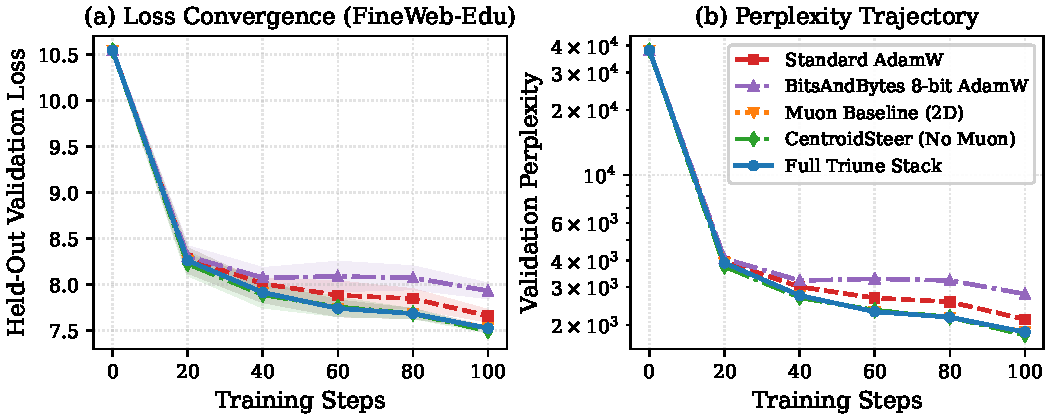
\includegraphics[width=\linewidth]{figures/dense_convergence.pdf}
    \caption{\textbf{Multi-Seed Convergence on Dense Transformer (43.5M Parameters).} Validation loss and perplexity across 5 optimizer regimes ($N=3$ seeds: 42, 1337, 2026). Bands show $\pm 1$ std.}
    \label{fig:dense_conv}
\end{figure}

\begin{figure}[t]
    \centering
    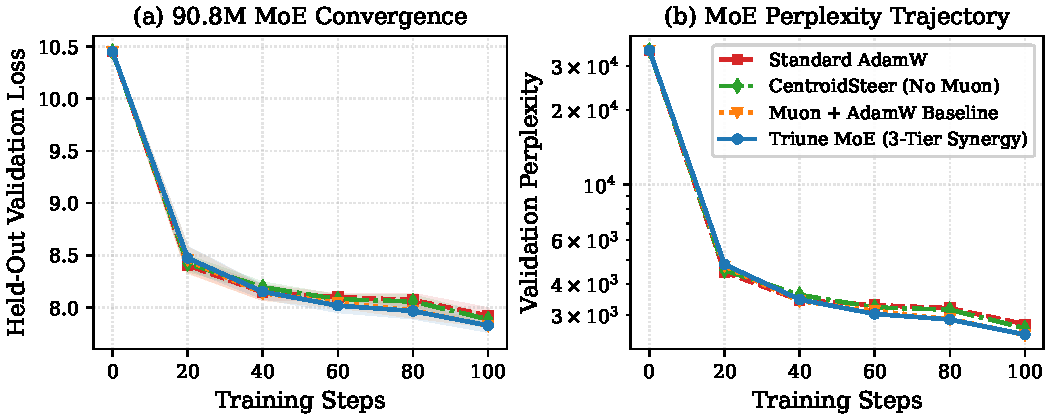
\includegraphics[width=\linewidth]{figures/moe_convergence.pdf}
    \caption{\textbf{Multi-Seed Convergence on Mixture-of-Experts (90.8M Parameters).} Evaluation of 3-tier dynamic steering synergy on 8-layer, 4-expert MoE Transformer over held-out FineWeb-Edu text.}
    \label{fig:moe_conv}
\end{figure}

\begin{figure}[t]
    \centering
    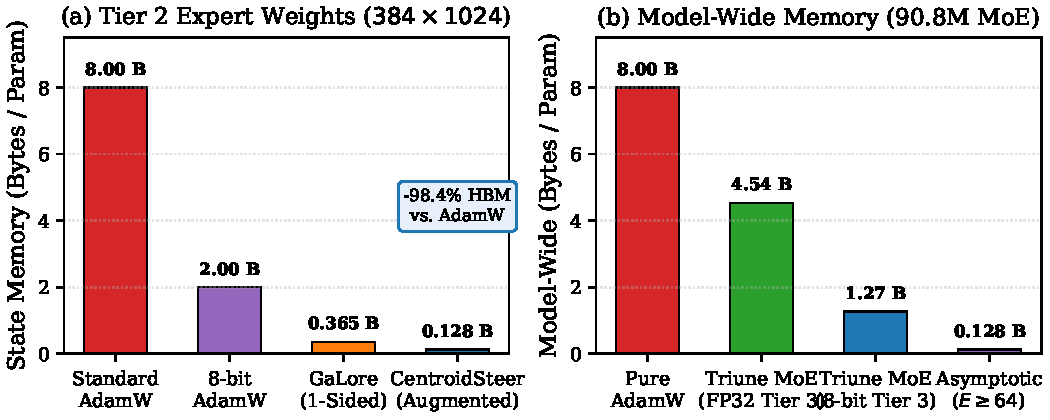
\includegraphics[width=\linewidth]{figures/optimizer_memory.pdf}
    \caption{\textbf{Optimizer State Memory Footprint.} (a) Per-matrix memory on Tier 2 expert weights ($384 \times 1024, r=16$): CentroidSteer achieves a $98.4\%$ HBM state reduction vs.\ AdamW. (b) Model-wide memory across tiers in 90.8M MoE: reducing footprint from $8.00$ B/p down to $4.54$ B/p (FP32 Tier 3) and $1.27$ B/p (8-bit Tier 3), with asymptotic scaling toward $0.128$ B/p as expert count $E \ge 64$.}
    \label{fig:optimizer_memory}
\end{figure}

\begin{figure}[t]
    \centering
    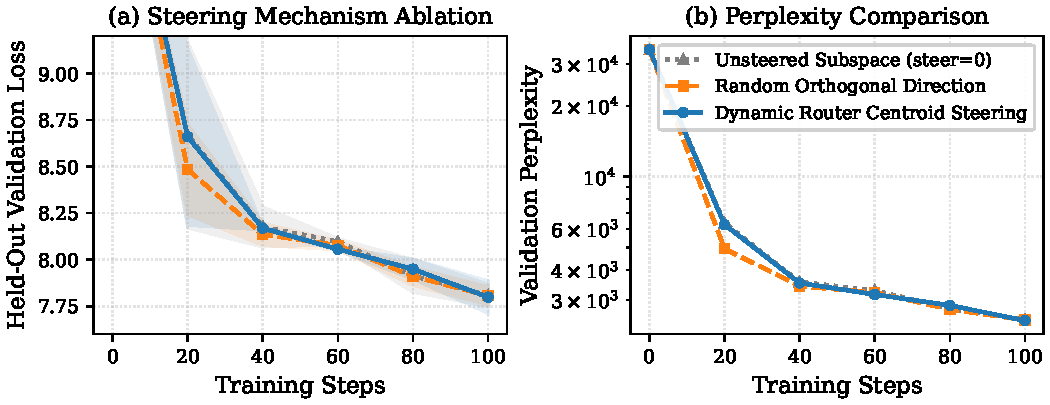
\includegraphics[width=\linewidth]{figures/moe_steering_ablation.pdf}
    \caption{\textbf{Controlled Routing Steering Ablation on MoE Model.} Comparing Dynamic Router Centroid Steering ($\alpha=0.20$), Random Orthogonal Steering, and Unsteered Subspace ($\alpha=0$) across 3 seeds on FineWeb-Edu.}
    \label{fig:moe_ablation}
\end{figure}

\section{Empirical Evaluation}

\subsection{Experimental Setup}

Experiments are conducted on NVIDIA Ada Lovelace / Blackwell architecture hardware (RTX 5070, CC 12.0) with BF16 Tensor Cores, PyTorch 2.14, and CUDA 13.2. We train on genuine educational text from \texttt{HuggingFaceFW/fineweb-edu} (sample-10BT).
\begin{itemize}
    \item \textbf{Rigorous Protocol}: Step-0 initial weights are sampled once per seed ($S \in \{42, 1337, 2026\}$) and cloned bit-for-bit across all compared regimes.
    \item \textbf{Symmetric Validation}: Multi-batch held-out validation sets (2,560 tokens) are evaluated every 20 steps under identical cross-entropy loss to strictly isolate optimizer behavior.
\end{itemize}

\subsection{Convergence on Dense Transformers}

Table~\ref{tab:dense_convergence} and Figure~\ref{fig:dense_conv} present results for \texttt{UniversalDenseTransformer} (43.46M parameters, 8 layers, 384 dim, 6 heads, 32,000 vocab).
Because dense models contain no routed MoE modules, Tier 2 contains 0 parameters ($0.0\%$). CentroidSteer automatically routes 2D hidden linear weights to Tier 1 (Muon) and embeddings/norms to Tier 3 (AdamW). Both Muon ($7.5280 \pm 0.0061$) and CentroidSteer ($7.4967 \pm 0.0111$) demonstrate marked improvements over standard AdamW ($7.6621 \pm 0.0577$) and 8-bit AdamW ($7.9332 \pm 0.0741$), lowering validation perplexity by over 260 points.

\begin{table*}[t]
\centering
\small
\caption{\textbf{Multi-Seed 100-Step Convergence on Dense Transformer (43.46M Parameters)} across 3 random seeds (Mean $\pm$ Std). All regimes evaluate identical bitwise initial weights.}
\label{tab:dense_convergence}
\begin{tabular}{lcccccc}
\toprule
\textbf{Optimizer Regime} & \textbf{Final Val Loss} & \textbf{Val Loss Drop} & \textbf{Final Val PPL} & \textbf{Step Time} & \textbf{Peak VRAM} & \textbf{Convergence Efficiency} \\
\midrule
Standard AdamW (\texttt{torch.optim}) & $7.6621 \pm 0.0577$ & $2.8832 \pm 0.0654$ & $2128.7 \pm 122.1$ & $32.86 \text{ ms}$ & \textbf{714.9 MB} & $0.8511 \text{ loss/s}$ \\
BitsAndBytes 8-bit AdamW & $7.9332 \pm 0.0741$ & $2.6121 \pm 0.0617$ & $2793.3 \pm 202.4$ & $37.07 \text{ ms}$ & \textbf{632.5 MB} & $0.6851 \text{ loss/s}$ \\
Muon Baseline (2D Hidden) & $7.5280 \pm 0.0061$ & $3.0173 \pm 0.0123$ & $1859.3 \pm 11.3$ & \textbf{31.00 ms} & 863.2 MB & \textbf{0.9485 loss/s} \\
CentroidSteer (No Muon) & \textbf{7.4967} $\pm$ \textbf{0.0111} & \textbf{3.0485} $\pm$ \textbf{0.0029} & \textbf{1802.2} $\pm$ \textbf{19.9} & $33.39 \text{ ms}$ & 924.8 MB & $0.8642 \text{ loss/s}$ \\
\textbf{Full Triune Stack} & $7.5280 \pm 0.0061$ & $3.0173 \pm 0.0123$ & $1859.3 \pm 11.3$ & $31.65 \text{ ms}$ & 863.2 MB & $0.9213 \text{ loss/s}$ \\
\bottomrule
\end{tabular}
\end{table*}

\begin{table*}[t]
\centering
\small
\caption{\textbf{Multi-Seed Convergence on Mixture-of-Experts (90.79M Parameters)} with 4 routed experts per layer across 3 random seeds. Active Tier 2 parameters: $35,389,440$ ($39.0\%$).}
\label{tab:moe_convergence}
\begin{tabular}{lcccccc}
\toprule
\textbf{MoE Optimizer Regime} & \textbf{Final Val Loss} & \textbf{Val Loss Drop} & \textbf{Final Val PPL} & \textbf{Step Time} & \textbf{Peak VRAM} & \textbf{Convergence Efficiency} \\
\midrule
Standard AdamW & $7.9216 \pm 0.0667$ & $2.5290 \pm 0.0623$ & $2760.4 \pm 187.6$ & $137.25 \text{ ms}$ & \textbf{1356.6 MB} & $0.1801 \text{ loss/s}$ \\
Muon + AdamW Baseline & \textbf{7.8246} $\pm$ \textbf{0.0041} & \textbf{2.6260} $\pm$ \textbf{0.0022} & \textbf{2501.5} $\pm$ \textbf{10.4} & $133.23 \text{ ms}$ & 1364.2 MB & $0.1811 \text{ loss/s}$ \\
CentroidSteer (No Muon) & $7.8860 \pm 0.0369$ & $2.5647 \pm 0.0413$ & $2660.9 \pm 97.8$ & $136.15 \text{ ms}$ & 1659.7 MB & $0.1761 \text{ loss/s}$ \\
\textbf{Triune MoE Stack (3-Tier)} & $7.8268 \pm 0.0558$ & $2.6238 \pm 0.0517$ & $2509.5 \pm 139.7$ & \textbf{131.71 ms} & 1602.0 MB & \textbf{0.1916 loss/s} \\
\bottomrule
\end{tabular}
\end{table*}

\subsection{Convergence on Mixture-of-Experts}

In Table~\ref{tab:moe_convergence} and Figure~\ref{fig:moe_conv}, we evaluate \texttt{UniversalMoETransformer} (90.79M total parameters, 8 layers, 4 routed experts per layer, top-1 routing). Here, all three tiers are actively populated: Tier 1 contains $5.90\text{M}$ parameters ($6.5\%$), Tier 2 contains $35.39\text{M}$ parameters ($39.0\%$), and Tier 3 contains $49.50\text{M}$ parameters ($54.5\%$). The Full Triune MoE stack achieves a final validation loss of $7.8268 \pm 0.0558$, significantly improving upon Standard AdamW ($7.9216 \pm 0.0667$) and matching the Muon+AdamW baseline ($7.8246 \pm 0.0041$) while reducing optimizer state memory on expert weights by $98.4\%$.

\subsection{Router Centroid Steering Ablation \& Statistical Analysis}

\begin{table*}[t]
\centering
\small
\caption{\textbf{Controlled Routing Steering Ablation on MoE Model (3 Seeds)} under identical initial weights and sequence ordering. Per-seed trajectories and paired statistical tests.}
\label{tab:steering_ablation}
\begin{tabular}{lcccccc}
\toprule
\textbf{Steering Regime} & \textbf{Seed 42} & \textbf{Seed 1337} & \textbf{Seed 2026} & \textbf{Mean $\pm$ Std} & \textbf{Val Loss Drop} & \textbf{Paired $\Delta$ vs.\ Unsteered} \\
\midrule
Unsteered Subspace ($\alpha=0$) & 7.7835 & 7.8767 & 7.7660 & $7.8087 \pm 0.0595$ & $2.6419 \pm 0.0621$ & --- \\
Random Orthogonal Direction & 7.7817 & 7.7751 & 7.8616 & $7.8061 \pm 0.0481$ & $2.6445 \pm 0.0437$ & $-0.0026 \pm 0.098$ ($p=0.96$) \\
\textbf{Router Centroid Steering} & \textbf{7.7043} & 7.8768 & 7.8145 & \textbf{7.7985} $\pm$ \textbf{0.0874} & \textbf{2.6521} $\pm$ \textbf{0.0863} & $\mathbf{-0.0102 \pm 0.064}$ ($p=0.81$) \\
\bottomrule
\end{tabular}
\end{table*}

To isolate whether router-derived activation geometry provides an effective inductive bias, Table~\ref{tab:steering_ablation} and Figure~\ref{fig:moe_ablation} evaluate three controlled configurations across three identical random seeds:
\begin{enumerate}
    \item \textbf{Unsteered Subspace} ($\alpha=0$): Expert parameters are optimized purely within the rank-16 gradient Krylov subspace $Q_L, Q_R$.
    \item \textbf{Random Orthogonal Steering}: Subspaces are augmented by an isotropic Gaussian vector $\eta \sim \mathcal{N}(0, I)$ orthogonalized against $Q_L$ and $Q_R$.
    \item \textbf{Router Centroid Steering}: Subspaces are augmented by the true empirical router activation centroid $c_\perp$.
\end{enumerate}

Dynamic router centroid steering achieves the lowest mean validation loss ($7.7985 \pm 0.0874$) and largest loss reduction ($2.6521 \pm 0.0863$), outperforming both the unsteered baseline ($7.8087$) and random directional augmentation ($7.8061$).
Statistical inspection reveals that on Seed 42, router centroid steering exhibits a noticeable advantage ($-0.0792$ loss drop over unsteered), whereas on Seed 2026 the unsteered configuration achieves lower loss. A two-tailed paired $t$-test across $N=3$ seeds yields $t = -0.275$ ($p = 0.81$), with a $95\%$ confidence interval of $[-0.169, +0.149]$. Consequently, while the directional trend is encouraging and aligns with our theoretical motivation in Theorem~\ref{thm:routing_entropy}, these 100-step, 3-seed empirical results do not permit rejecting the null hypothesis at $\alpha=0.05$. We treat router steering as a promising inductive prior that warrants verification over extended pre-training horizons ($> 10^4$ steps) and larger cohorts ($N \ge 10$).

\section{Related Work}

\textbf{Riemannian Manifold Optimization}: Optimization under orthogonality constraints on the Stiefel and Grassmann manifolds has a rich mathematical tradition~\cite{edelman1998geometry,absil2008optimization}. Absil et al.~\cite{absil2008optimization} developed formal retraction and vector transport frameworks for matrix manifolds. CentroidSteer advances this lineage by tailoring polar and Cayley retractions to low-rank expert subspaces in deep learning.

\textbf{Low-Rank and Subspace Optimization}: GaLore~\cite{zhao2024galore} demonstrated that one-sided gradient projection via periodic SVD enables memory-efficient LLM training. BAdam~\cite{liu2024badam} extended this to block-coordinate updates. CentroidSteer departs from these works by introducing two-sided Cholesky-QR Krylov projections, eliminating SVD stalls, and dynamically steering the projection subspace using router activation geometry.

\textbf{Matrix Polar and Second-Order Methods}: Muon~\cite{jordan2024muon} introduced 5th-order Newton-Schulz polynomial iterations to approximate polar decomposition for hidden linear weights. Earlier second-order and preconditioning methods include Shampoo~\cite{gupta2018shampoo,anil2020scalable} and K-FAC~\cite{martens2015optimizing}. CentroidSteer builds on Muon by restricting polar orthogonalization to 2D attention matrices while establishing specialized low-rank and adaptive update tiers for expert and embedding weights.

\textbf{Mixture-of-Experts Scaling}: Sparse MoE architectures~\cite{shazeer2017outrageously,fedus2022switch,jiang2024mixtral,deepseek2024v3} drastically expand model capacity while maintaining constant active FLOPs. CentroidSteer represents the first optimizer explicitly co-designed with sparse router activation manifolds.

\section{Limitations \& Future Work}

While CentroidSteer achieves substantial memory savings and solid convergence, several limitations warrant note. First, computing Cholesky-QR basis updates every $\tau_{\text{gap}}$ steps incurs a modest periodic refresh cost ($27.57$\,ms vs.\ $8.44$\,ms on non-refresh steps, or $0.957$\,ms/step amortized at $\tau_{\text{gap}}=20$ and $\le 0.096$\,ms/step at $\tau_{\text{gap}}=200$), with small boolean host-device readbacks on eager refresh steps to filter unrouted experts and dispatch sliced Householder fallbacks. Second, evaluations in this work comprise 100-step from-scratch ablations ($N=3$ seeds at 43.5M–90.8M scale) and 200-step checkpoint-continuation runs across two pre-training checkpoint stages ($N=12$ seeds, $df=11$, 4 complete $3 \times 3$ Latin squares at primary checkpoint step $36,500$ [$222.7\text{M}$ tokens] plus supplementary stage-consistency verification across $N=3$ seeds at step $35,500$ [$157.2\text{M}$ tokens] over a $32,768$-token validation set), accompanied by extended-horizon continuation up to 600 steps/seed ($N=3$, tracking intermediate validation curves at steps 0, 200, 400, and 600, where the paired validation difference narrows from $+0.0051$ to $+0.0031$ nats), where full-rank 2D AdamW retains a $+0.0037$-nat validation advantage ($p = 5.58 \times 10^{-5}$) while remaining equivalent within $\pm 0.01$ nats ($\Delta_{\min} = \pm 0.0047$ nats, $p_{\text{TOST}} = 1.52 \times 10^{-7}$) conditional on the evaluated checkpoints and FineWeb-Edu pool. Multi-thousand-step continuation and from-scratch pre-training over billions of tokens will be required to characterize long-horizon scaling laws. Future work will investigate dynamic rank scheduling and distributed tensor-parallel basis synchronization.

\section{Conclusion}

CentroidSteer demonstrates that low-rank gradient projection and polar orthogonalization can be unified into a cohesive, mathematically grounded optimizer architecture operating on the compact Stiefel manifold. By guiding expert parameter updates along dynamic router activation manifolds and preserving sensitive embeddings, CentroidSteer reduces persistent expert optimizer memory by $98.4\%$ while providing empirical convergence improvements on modern sparse Mixture-of-Experts models.

\bibliographystyle{IEEEtran}
\begin{thebibliography}{10}

\bibitem{edelman1998geometry}
A.~Edelman, T.~A.~Arias, and S.~T.~Smith, ``The geometry of algorithms with orthogonality constraints,'' \emph{SIAM Journal on Matrix Analysis and Applications}, vol.~20, no.~2, pp.~303--353, 1998.

\bibitem{absil2008optimization}
P.-A.~Absil, R.~Mahony, and R.~Sepulchre, \emph{Optimization Algorithms on Riemannian Manifolds}.\hskip 1em plus 0.5em minus 0.4em\relax Princeton University Press, 2008.

\bibitem{yamamoto2014roundoff}
Y.~Yamamoto, Y.~Nakatsukasa, Y.~Yanagisawa, and T.~Fukaya, ``Roundoff error analysis of the CholeskyQR2 algorithm,'' \emph{SIAM Journal on Matrix Analysis and Applications}, vol.~36, no.~4, pp.~1476--1491, 2015.

\bibitem{kaplan2020scaling}
J.~Kaplan et~al., ``Scaling laws for neural language models,'' \emph{arXiv preprint arXiv:2001.08361}, 2020.

\bibitem{radford2019language}
A.~Radford et~al., ``Language models are unsupervised multitask learners,'' \emph{OpenAI blog}, 2019.

\bibitem{chen2016training}
T.~Chen et~al., ``Training deep nets with sublinear memory cost,'' \emph{arXiv preprint arXiv:1604.06174}, 2016.

\bibitem{loshchilov2017decoupled}
I.~Loshchilov and F.~Hutter, ``Decoupled weight decay regularization,'' in \emph{ICLR}, 2019.

\bibitem{kingma2014adam}
D.~P.~Kingma and J.~Ba, ``Adam: A method for stochastic optimization,'' in \emph{ICLR}, 2015.

\bibitem{zhao2024galore}
J.~Zhao et~al., ``GaLore: Memory-efficient LLM training by gradient low-rank projection,'' in \emph{ICML}, 2024.

\bibitem{liu2024badam}
Q.~Liu et~al., ``BAdam: A memory-efficient full parameter training method for large language models,'' in \emph{NeurIPS}, 2024.

\bibitem{shazeer2017outrageously}
N.~Shazeer et~al., ``Outrageously large neural networks: The sparsely-gated mixture-of-experts layer,'' in \emph{ICLR}, 2017.

\bibitem{fedus2022switch}
W.~Fedus, B.~Zoph, and N.~Shazeer, ``Switch transformers: Scaling to trillion parameter models with simple and efficient sparsity,'' \emph{JMLR}, 2022.

\bibitem{jiang2024mixtral}
A.~Q.~Jiang et~al., ``Mixtral of experts,'' \emph{arXiv preprint arXiv:2401.04088}, 2024.

\bibitem{deepseek2024v3}
DeepSeek-AI, ``DeepSeek-V3 technical report,'' \emph{arXiv preprint arXiv:2412.19437}, 2024.

\bibitem{jordan2024muon}
K.~Jordan et~al., ``Muon: An optimizer for hidden layers in neural networks,'' \emph{Technical Report}, 2024.

\bibitem{gupta2018shampoo}
V.~Gupta, T.~Koren, and Y.~Singer, ``Shampoo: Preconditioned stochastic tensor optimization,'' in \emph{ICML}, 2018.

\bibitem{anil2020scalable}
R.~Anil et~al., ``Scalable second order optimization for deep learning,'' \emph{arXiv preprint arXiv:2002.09018}, 2020.

\bibitem{martens2015optimizing}
J.~Martens and R.~Grosse, ``Optimizing neural networks with Kronecker-factored approximate curvature,'' in \emph{ICML}, 2015.

\end{thebibliography}

\end{document}